%
%  progress-presentation.tex
%  src
%
%  Created by Illya Starikov on 09/16/17.
%  Copyright 2017. Illya Starikov. All rights reserved.
%

% \documentclass[notes,xcolor=dvipsnames]{beamer}       % print frame + notes
% \documentclass[notes=only,xcolor=dvipsnames]{beamer}  % only notes
\documentclass[xclolor=dvipsnames]{beamer}            % only frames
%\documentclass[handout,xclolor=dvipsnames]{beamer}    % only frames, no pauses
\usepackage{soul,graphics}

\usepackage{amssymb,amsmath,verbatim,graphicx,microtype,upquote,units,booktabs,akkwidepage}

\newcommand{\chapterNumber}[1]{
    \setcounter{section}{#1}
    \addtocounter{section}{-1}
}
\title{Bartending (Presentation \#9)}
\subtitle{Special Topics (CS3001)}
\author{Illya Starikov}
\date{Sometimes In The Future}
\institute{Missouri University of Science and Technology}

\begin{document}
\begin{darkframes}
    \maketitle

    \begin{frame}
        \frametitle{A Brief Introduction}

        \begin{quote}
            Disclaimer: I am 21.
        \end{quote}
    \end{frame}

    \begin{frame}
        \frametitle{A Brief Introduction}

        I got onto a streak of cool bartending videos earlier in the semesters, such as:

        \begin{itemize}
            \item \href{https://www.youtube.com/watch?v=60GJ0dJ1xmE}{This one.}
            \item \href{https://www.youtube.com/watch?v=KRNBLQYTwz4}{This one.}
            \item \href{https://www.youtube.com/watch?v=AEx6ajEeGVg}{This one.}
        \end{itemize}

        Inspired by this, I wanted to become a decent bartender.

        First, I knew I had to get some supplies.
    \end{frame}

    \begin{frame}
        \frametitle{A Brief Introduction}
        \subtitle{Supplies}

        \begin{figure}[H]
            \centering
            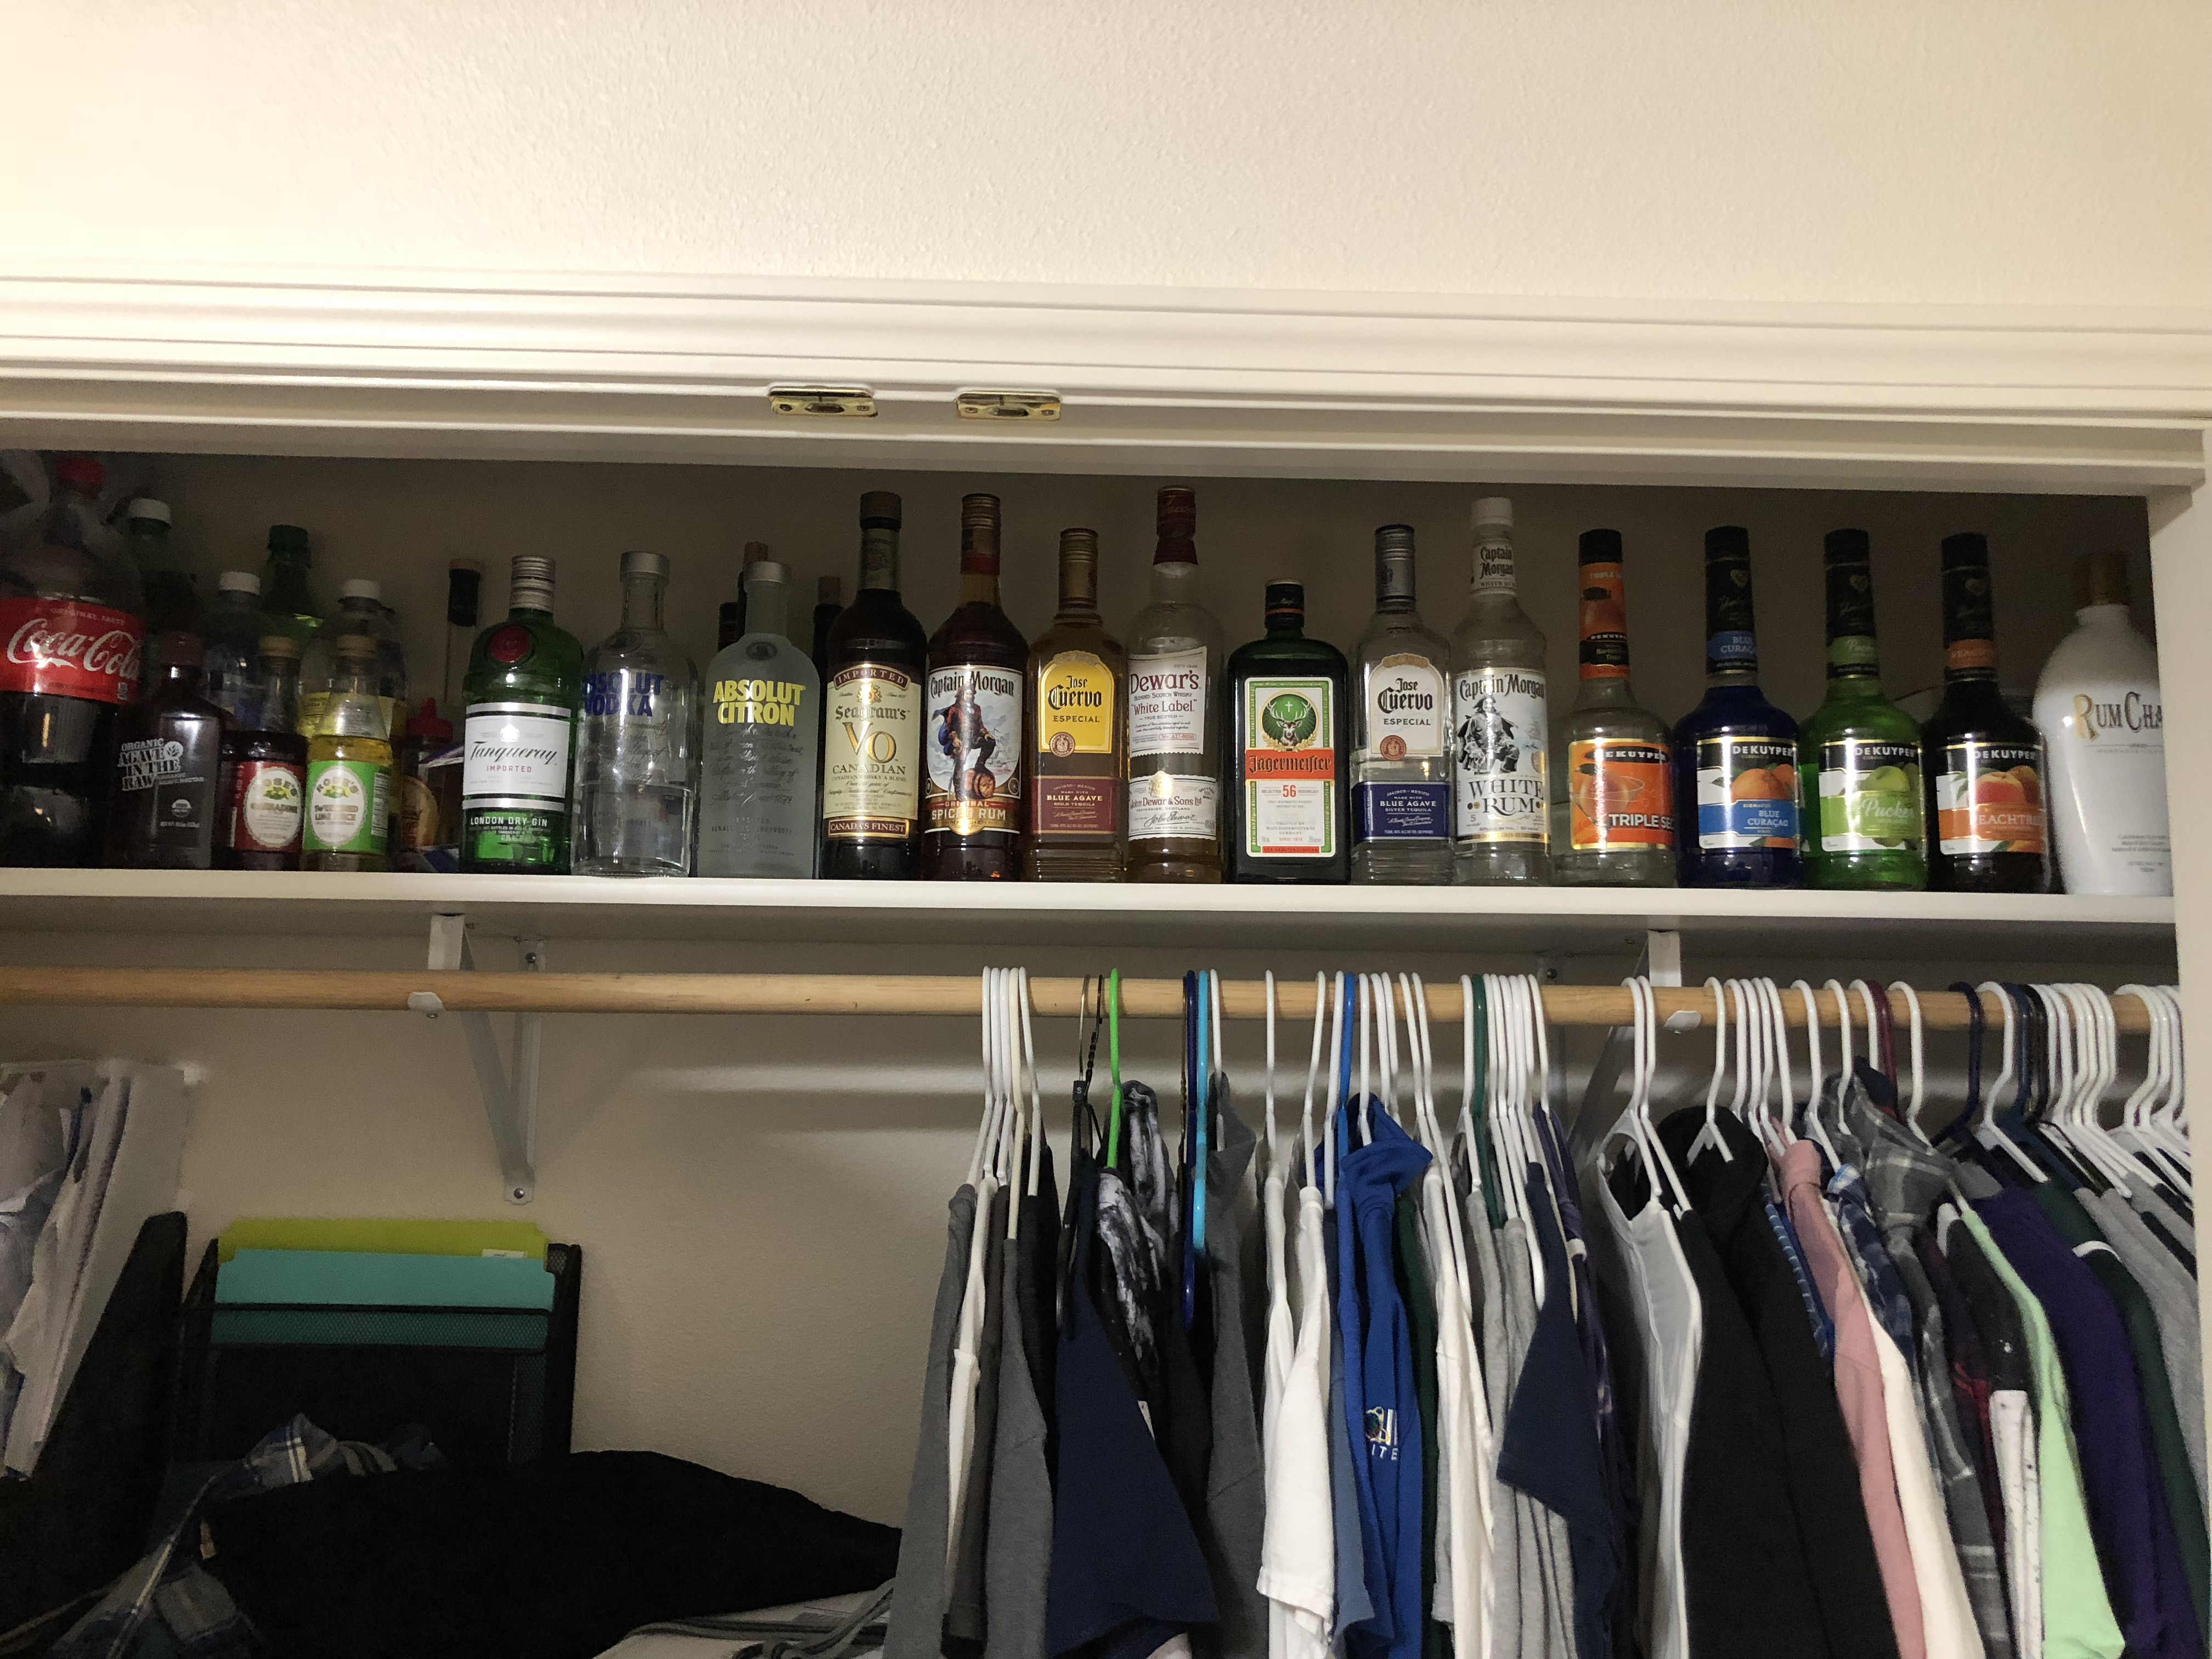
\includegraphics[width=.8\linewidth]{assets/alcohol.jpg}
            \caption{Some of the Alcohol Necessary For Bartending}
            \label{fig:alcohol}
        \end{figure}
    \end{frame}

    \begin{frame}
        \frametitle{A Brief Introduction}
        \subtitle{Supplies}

        \begin{figure}[H]
            \centering
            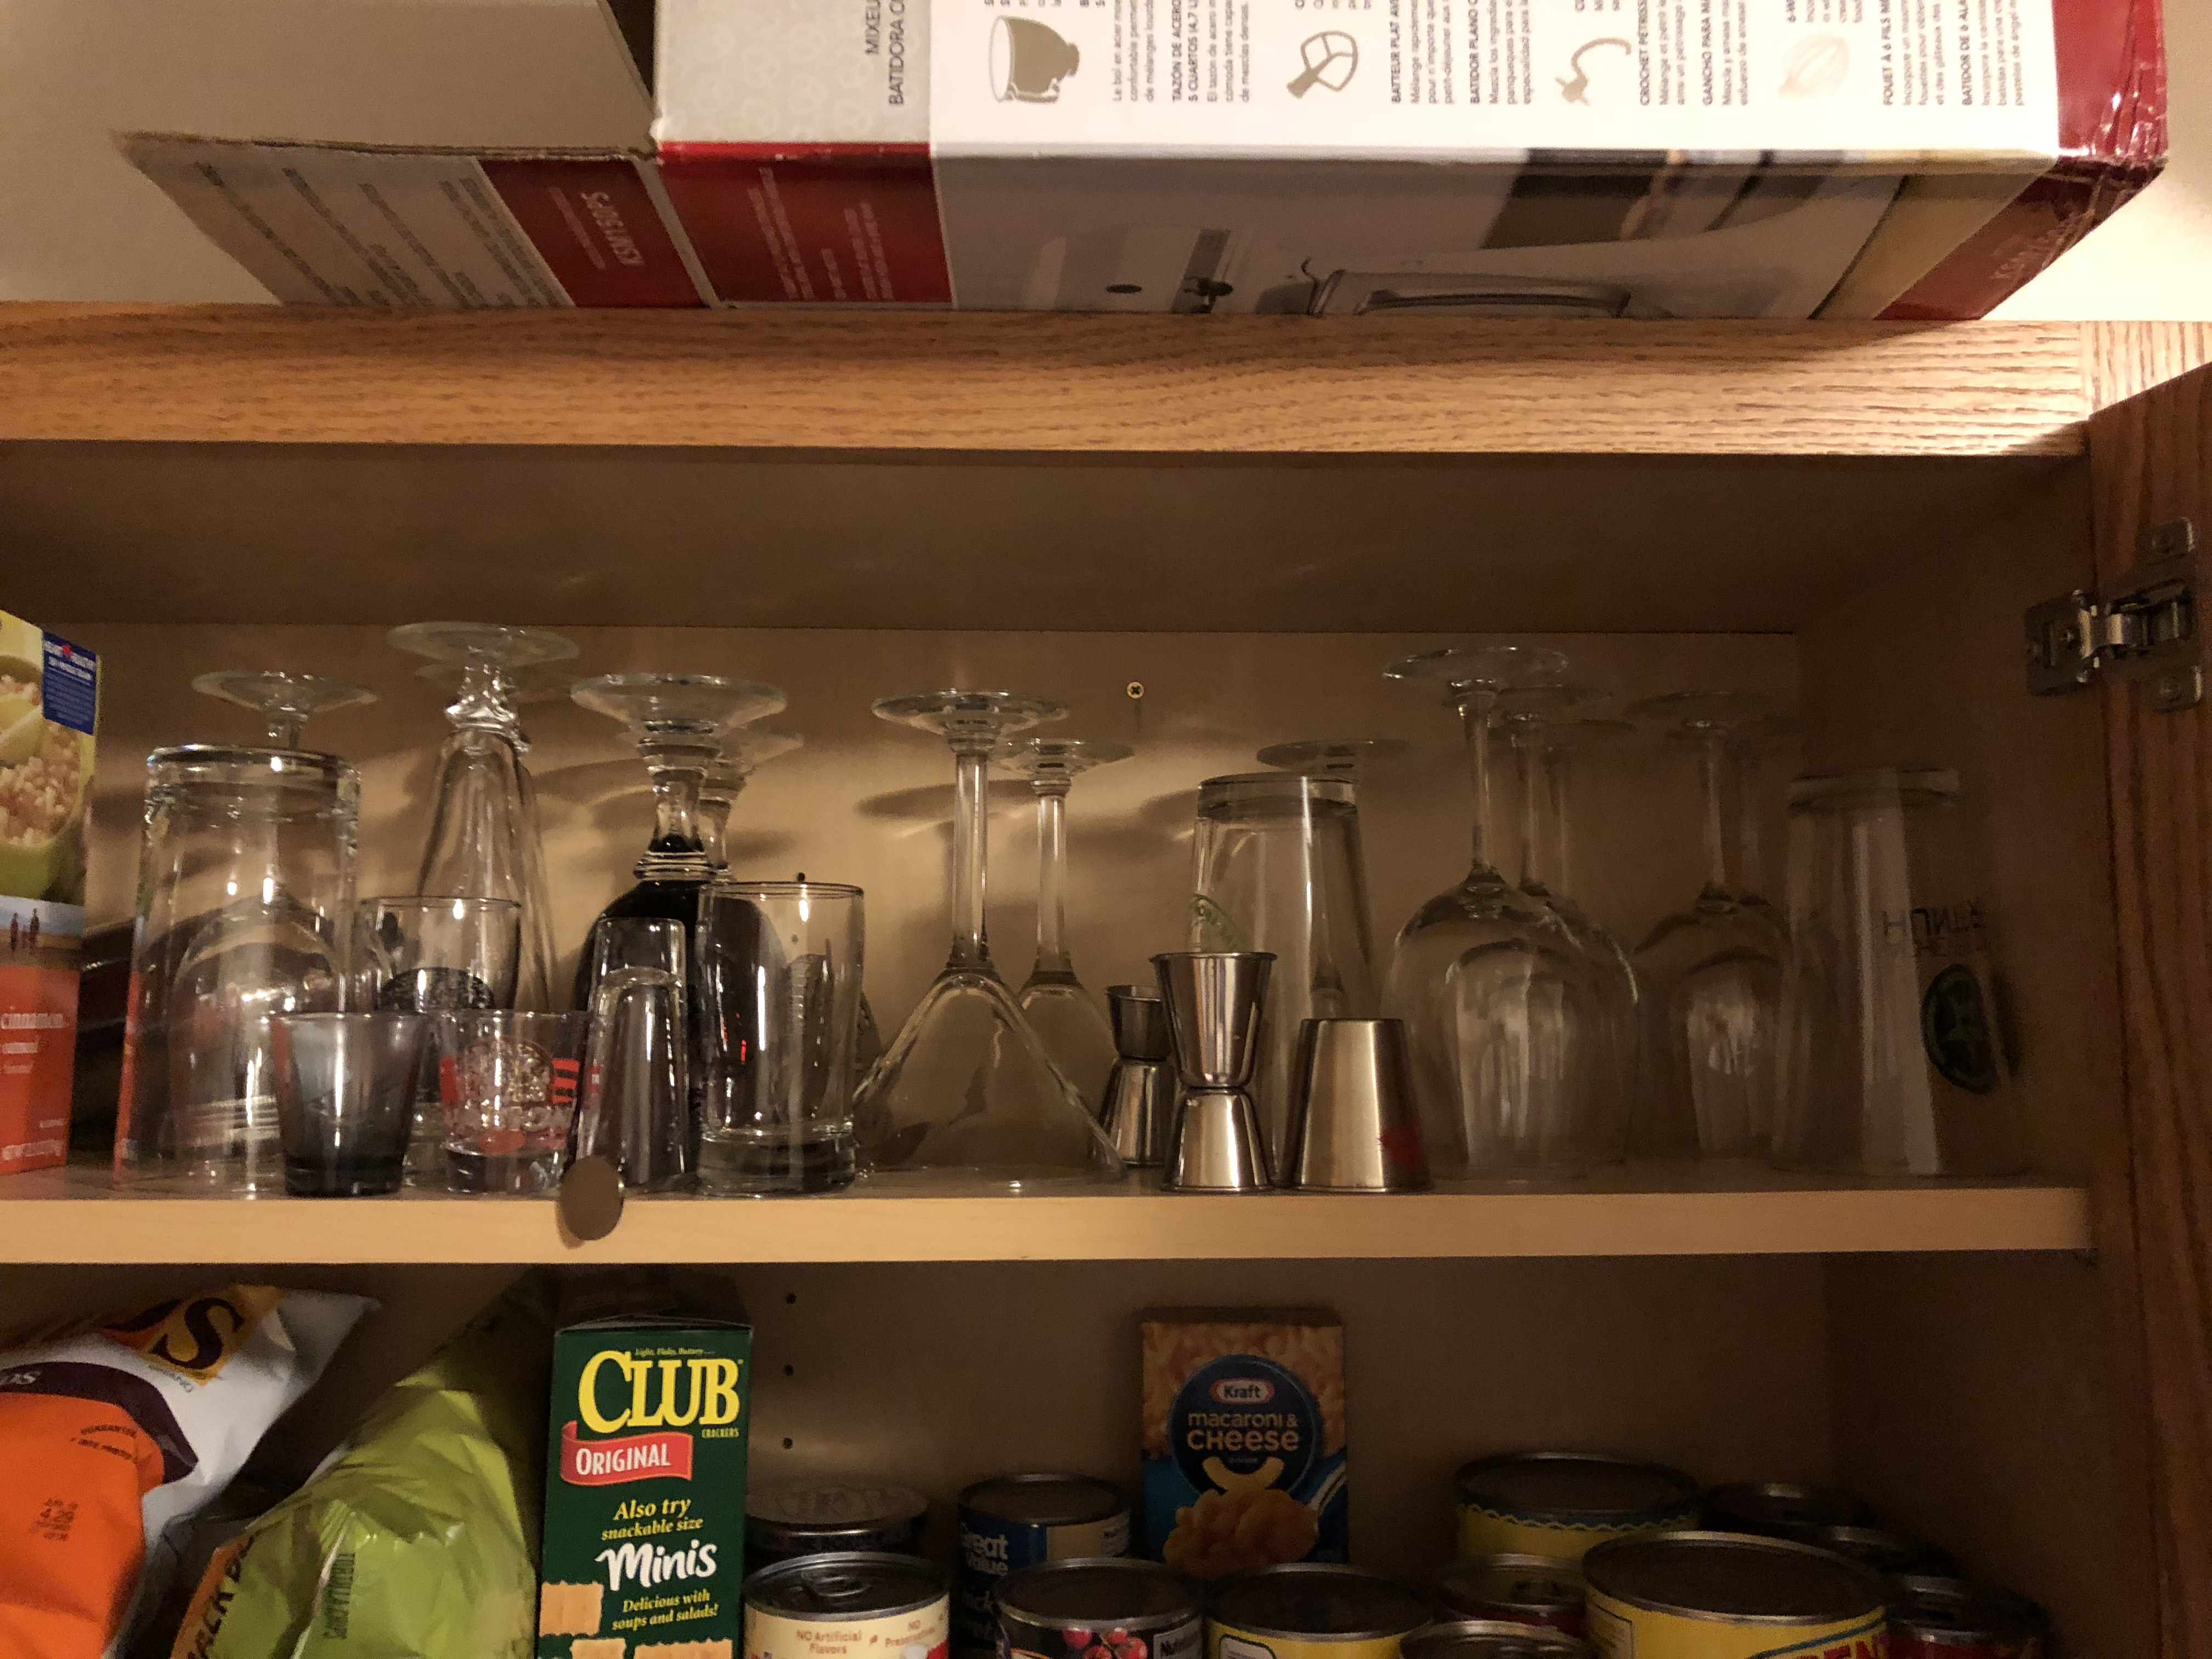
\includegraphics[width=.8\linewidth]{assets/tools.jpg}
            \caption{Some of the Tools Necessary For Bartending}
            \label{fig:alcohol}
        \end{figure}
    \end{frame}

    \begin{frame}
        \frametitle{Prior Knowledge}

        \begin{itemize}
            \item I did not have much prior knowledge to this.
        \end{itemize}
    \end{frame}

    \begin{frame}
        \frametitle{Goals}

        \begin{itemize}
            \item To become well acquainted with some of the more famous cocktails and what is in them.
            \item To become make these drinks with some flair.
        \end{itemize}
    \end{frame}

    \begin{frame}
        \frametitle{Resources}

        \begin{itemize}
            \item To learn the mechanics of bartending, a lot of it came from practice and YouTube.
                \begin{itemize}
                    \item \href{https://www.youtube.com/watch?v=adlWwvHtGVA}{How to pour.}
                    \item \href{https://www.youtube.com/watch?v=mNYxSepBHJs}{How to flip pour.}
                    \item \href{https://www.youtube.com/watch?v=s4weXtuax8Q}{How to set up a bar.}
                \end{itemize}

            \item I also picked up a book to passively read: \href{https://www.amazon.com/Liquid-Intelligence-Science-Perfect-Cocktail-ebook/dp/B00J8R3KOE}{Liquid Intelligence}.
        \end{itemize}
    \end{frame}

    \begin{frame}
        \frametitle{Goal Accomplishment}

        \begin{itemize}
            \item I have learned how to make several of the famous cocktails relatively well.

            \item Some of them were very easy.
                \begin{itemize}
                    \item Screw Driver
                    \item Fuzzy Naval
                    \item Sex on the Beach
                \end{itemize}

            \item Some of them were more difficult to make.\footnote{Not hard to make, but hard to get correct.}
                \begin{itemize}
                    \item Mojitos
                    \item Mai Tai
                    \item Martini
                \end{itemize}
        \end{itemize}
    \end{frame}

    \begin{frame}
        \frametitle{Goal Accomplishment}

        \begin{itemize}
            \item I also learned how to do some of the cool bar tricks in the previous videos.
        \end{itemize}
    \end{frame}


    \begin{frame}
        \frametitle{Lessons Learned}

        Aside from the cocktails I made, there were some lessons I learned.

        \begin{itemize}
            \item The real difference between shaken and stirred and how it effects a drink.
            \item How much ice can effect a cocktail.
            \item What different liquor combinations can be combined to produce different flavors.
        \end{itemize}

    \end{frame}

    \begin{frame}
        \frametitle{In Closing}

        All question, comments, and insults can be directed towards me:

        \begin{center}
            \begin{description}
                \item[\faComment] \href{mailto:starikov@mst.edu}{starikov@mst.edu}
                \item[\faLinkedin] \href{https://www.linkedin.com/in/illyastarikov/}{Illya Starikov}
                \item[\faGithub] \href{https://github.com/IllyaStarikov/}{Illya Starikov}
                \item[\faRss] \href{https://freneticarray.com/}{FreneticArray.com}
            \end{description}
        \end{center}
    \end{frame}
\end{darkframes}
\end{document}
